\documentclass[a4paper,12pt]{article}
\setlength{\headheight}{14.49998pt}
\addtolength{\topmargin}{-2.49998pt}
% Packages
\usepackage[utf8]{inputenc}
\usepackage[T1]{fontenc}
\usepackage[portuguese]{babel}
\usepackage{siunitx}
\usepackage{booktabs}
\usepackage{amsfonts}
\usepackage{listings}
\usepackage{graphicx,url}
\usepackage{subfigure}
\usepackage{xcolor}
\usepackage{hyperref}
\usepackage{float}
\usepackage{booktabs}
\usepackage{fvextra}
\usepackage{graphicx}
\usepackage{amsmath}
\usepackage{geometry}
\usepackage{algorithm}
\usepackage{algorithmic}
\usepackage{fancyhdr}
\usepackage{setspace}
\usepackage{titlesec}  % For title formatting
\geometry{margin=0.8in}
\setstretch{1.5}
\usepackage{amssymb}
\usepackage{enumitem}




\newcommand{\bigO}{\mathcal{O}}
\newcommand{\blue}{\color{blue}} 
\newcommand{\red}{\color{red}} 
\newcommand{\R}{\mathbb{R}}
\usepackage{cancel}
\renewcommand{\CancelColor}{\color{red}}

\usepackage{listings}
\usepackage{xcolor} %cores usadas no lstdefinestyle
\definecolor{codegreen}{rgb}{0,0.6,0}
\definecolor{codegray}{rgb}{0.5,0.5,0.5}
\definecolor{codepurple}{rgb}{0.58,0,0.82}
\definecolor{backcolour}{rgb}{0.95,0.95,0.92}
\lstdefinestyle{mystyle}{
	language = Python,
	backgroundcolor=\color{backcolour},
	commentstyle=\color{codegreen},
	keywordstyle=\color{magenta},
	numberstyle=\tiny\color{codegray},
	stringstyle=\color{codepurple},
	basicstyle=\ttfamily\footnotesize,
	breakatwhitespace=false,         
	breaklines=true,                 
	captionpos=b,                    
	keepspaces=true,                 
	numbers=left,                    
	numbersep=5pt,                  
	showspaces=false,                
	showstringspaces=false,
	showtabs=false,                  
	tabsize=2,
    literate={á}{{\'a}}1 {ã}{{\~a}}1 {é}{{\'e}}1  {á}{{\'a}}1  {é}{{\'e}}1  {í}{{\'i}}1 {ó}{{\'o}}1  {ú}{{\'u}}1
    {Á}{{\'A}}1  {É}{{\'E}}1  {Í}{{\'I}}1 {Ó}{{\'O}}1  {Ú}{{\'U}}1
      {à}{{\`a}}1  {è}{{\`e}}1  {ì}{{\`i}}1 {ò}{{\`o}}1  {ù}{{\`u}}1
      {À}{{\`A}}1  {È}{{\`E}}1  {Ì}{{\`I}}1 {Ò}{{\`O}}1  {Ù}{{\`U}}1
      {ä}{{\"a}}1  {ë}{{\"e}}1  {ï}{{\"i}}1 {ö}{{\"o}}1  {ü}{{\"u}}1
      {Ä}{{\"A}}1  {Ë}{{\"E}}1  {Ï}{{\"I}}1 {Ö}{{\"O}}1  {Ü}{{\"U}}1
      {â}{{\^a}}1  {ê}{{\^e}}1  {î}{{\^i}}1 {ô}{{\^o}}1  {û}{{\^u}}1
      {Â}{{\^A}}1  {Ê}{{\^E}}1  {Î}{{\^I}}1 {Ô}{{\^O}}1  {Û}{{\^U}}1
      {œ}{{\oe}}1  {Œ}{{\OE}}1  {æ}{{\ae}}1 {Æ}{{\AE}}1  {ß}{{\ss}}1
      {ẞ}{{\SS}}1  {ç}{{\c{c}}}1 {Ç}{{\c{C}}}1 {ø}{{\o}}1  {Ø}{{\O}}1
      {å}{{\aa}}1  {Å}{{\AA}}1  {ã}{{\~a}}1  {õ}{{\~o}}1 {Ã}{{\~A}}1
      {Õ}{{\~O}}1  {ñ}{{\~n}}1  {Ñ}{{\~N}}1  {¿}{{?`}}1  {¡}{{!`}}1
      {°}{{\textdegree}}1 {º}{{\textordmasculine}}1 {ª}{{\textordfeminine}}1
      {£}{{\pounds}}1  {©}{{\copyright}}1  {®}{{\textregistered}}1
      {«}{{\guillemotleft}}1  {»}{{\guillemotright}}1  {Ð}{{\DH}}1  {ð}{{\dh}}1
      {Ý}{{\'Y}}1    {ý}{{\'y}}1    {Þ}{{\TH}}1    {þ}{{\th}}1    {Ă}{{\u{A}}}1
      {ă}{{\u{a}}}1  {Ą}{{\k{A}}}1  {ą}{{\k{a}}}1  {Ć}{{\'C}}1    {ć}{{\'c}}1
      {Č}{{\v{C}}}1  {č}{{\v{c}}}1  {Ď}{{\v{D}}}1  {ď}{{\v{d}}}1  {Đ}{{\DJ}}1
      {đ}{{\dj}}1    {Ė}{{\.{E}}}1  {ė}{{\.{e}}}1  {Ę}{{\k{E}}}1  {ę}{{\k{e}}}1
      {Ě}{{\v{E}}}1  {ě}{{\v{e}}}1  {Ğ}{{\u{G}}}1  {ğ}{{\u{g}}}1  {Ĩ}{{\~I}}1
      {ĩ}{{\~\i}}1   {Į}{{\k{I}}}1  {į}{{\k{i}}}1  {İ}{{\.{I}}}1  {ı}{{\i}}1
      {Ĺ}{{\'L}}1    {ĺ}{{\'l}}1    {Ľ}{{\v{L}}}1  {ľ}{{\v{l}}}1  {Ł}{{\L{}}}1
      {ł}{{\l{}}}1   {Ń}{{\'N}}1    {ń}{{\'n}}1    {Ň}{{\v{N}}}1  {ň}{{\v{n}}}1
      {Ő}{{\H{O}}}1  {ő}{{\H{o}}}1  {Ŕ}{{\'{R}}}1  {ŕ}{{\'{r}}}1  {Ř}{{\v{R}}}1
      {ř}{{\v{r}}}1  {Ś}{{\'S}}1    {ś}{{\'s}}1    {Ş}{{\c{S}}}1  {ş}{{\c{s}}}1
      {Š}{{\v{S}}}1  {š}{{\v{s}}}1  {Ť}{{\v{T}}}1  {ť}{{\v{t}}}1  {Ũ}{{\~U}}1
      {ũ}{{\~u}}1    {Ū}{{\={U}}}1  {ū}{{\={u}}}1  {Ů}{{\r{U}}}1  {ů}{{\r{u}}}1
      {Ű}{{\H{U}}}1  {ű}{{\H{u}}}1  {Ų}{{\k{U}}}1  {ų}{{\k{u}}}1  {Ź}{{\'Z}}1
      {ź}{{\'z}}1    {Ż}{{\.Z}}1    {ż}{{\.z}}1    {Ž}{{\v{Z}}}1 %comando literate para usar acento no lstlisting
}
\lstset{style=mystyle}


% Header and Footer
\pagestyle{fancy}
\fancyhf{}
\fancyhead[L]{Regiões de Estabilidade e Computação Paralela}
\fancyhead[R]{\thepage}

% Title Formatting
\titleformat{\section}{\normalfont\Large\bfseries}{\thesection}{1em}{}

% Cover Page
\title{
    \vspace{2cm} % Adjust vertical space
    
\includegraphics[width=0.55\textwidth]{Figuras/logo_icmc.png} \\ % Add your logo here (change "logo.png" to the actual filename)
    \vspace{1cm} % Adjust vertical space after the logo
    \textbf{\Huge Assignment 2} \\
    \vspace{1cm} % Adjust vertical space
    \large Regiões de Estabilidade de Métodos Numéricos para Equações Diferenciais com computação paralela \\
    \vspace{0.5cm}\thanks{Este trabalho foi realizado com auxílio de recurso computacional do cluster Euler\\Todos os códigos utilizados na elaboração deste trabalho estão disponíveis no GitHub: \url{https://github.com/victorcunha94/hcp_for_edp}}
    
}
\author{Bruno Dalcantoni Cozac \\
        Gabriel de Oliveira Bispo \\
        Deyvisson Nascimento Garcês (17415244) \\
        Victor Matheus da Cunha Santos (13279534) }

\date{\today}

\begin{document}

% Title Page
\maketitle
\thispagestyle{empty}
\newpage

% Table of Contents
% Start page numbering from the Table of Contents
\tableofcontents
\newpage

\section{Equações Diferenciais}

\begin{equation*}
    \left\{
\begin{array}{cc}
     \mathbf{u}'(t) = & \mathbf{f}(u(t),t)\\
     \mathbf{u}(0) = & \eta(t) 
\end{array}
    \right.
\end{equation*}

\subsection{Métodos baseados em expansões de Série de Taylor}



\subsection{Exercício 01}
Considere o problema particular, 

\begin{equation*}\label{eq:caso1}
    u'(t) = -\lambda u(t), \quad u(0) = 1
\end{equation*}
com $\lambda > 0$, cuja solução é $u(t) = e^{-\lambda t} $. Note que
\begin{equation*}
    \lim_{t\to\infty} u(t) = 0.
\end{equation*}
Quando aplicamos o método de progressivo na equação \eqref{eq:caso1}, obtemos
\begin{align*}
    U^{n + 1} = & ~ U^{n} + h f(U^{n},t_{n}) \\
    U^{n + 1} = & ~ U^{n} - h \lambda U^{n} 
\end{align*}
Podemos perceber que quando o passo temporal $n$ avança, tem-se uma fórmula obtida por recorrência
\begin{align*}
      U^{n + 1}  = & ~ (1 - h\lambda)^{n+1} ~ U^{0}.
\end{align*}


Para a solução aproximada, temos

\begin{equation*}
    \lim_{n \to \infty} U^{n} = 0 \quad \Longleftrightarrow \quad |1 - h\lambda| < 1.
\end{equation*}

Podemos perceber que não é possível escolher um $h$ arbitrário, para que a solução numérica convirja é preciso levar em consideração que o método impõe uma restrição sobre a escolha de $h$, 

\begin{align}
    |1 - h\lambda| < 1  & = |h\lambda - 1| < 1\\
     0 < h\lambda  \qquad \mbox{e} & \qquad 1 + h\lambda < 1
\end{align}

\section{Validação do código}
\begin{figure}[H]
\centering
\subfigure[Um filhote. \label{fig:euler_python}]{
\includegraphics[width=.38\textwidth]{Figuras/PYTHON/stability_basic_1threads.png}
} % end subfigure
\quad % dá um espaço entre as duas figuras.
\subfigure[Vários filhotes. \label{fig:euler_leveque}]{
\includegraphics[width=.4\textwidth]{Figuras/PYTHON/euler_leveque.png}
} % end subfigure
\caption{Comparação para validação do código}
\label{fig:euler_implicito}
\end{figure}



\section{Análise do algoritmo em Python: Sequencial vs Paralelo}

Nesta sessão discutimos a implementação do código em paralelo e a estratégia adotada. Utilizamos o compilador \textit{\href{https://numba.pydata.org/}{Numba}} e a estratégia por "blocos".

\subsection{Algoritmo}

\begin{algorithm}
\caption{Verificação de Estabilidade para um ponto \( z \)}
\label{alg:stability}
\begin{algorithmic}[1]
\STATE $U_n \gets [1, 0]$ \COMMENT{Inicialização $u_0 = 1 + 0i$}
\FOR{$n = 0$ to $T-1$}
    \STATE $U_{n+1} \gets \text{method\_one\_step}(U_n, z)$ \COMMENT{Iteração do método numérico}
    \STATE $U_n \gets U_{n+1}$
    \IF{$\|U_n\|_2 < \epsilon$}
        \RETURN 1 \COMMENT{Ponto Estável}
    \ELSIF{$\|U_n\|_2 > 1/\epsilon$}
        \RETURN 0 \COMMENT{Ponto Instável}
    \ENDIF
\ENDFOR
\RETURN 0.5 \COMMENT{Ponto Indeterminado}
\end{algorithmic}
\end{algorithm}

O algoritmo para determinar a estabilidade de um ponto \( z \) no plano complexo segue a lógica descrita no Algoritmo~\ref{alg:stability}. Inicializa-se a sequência \( u_0 = 1 \). Para cada iteração \( n \) (até um máximo de \( T \) iterações), calcula-se \( u_{n+1} \) aplicando-se uma iteração do método numérico (Euler Implícito) sob o parâmetro \( z \). A norma (módulo) de \( u_n \) é verificada a cada passo. Se a norma cair abaixo de uma tolerância \( \epsilon \), o ponto é considerado \textbf{estável} (convergente para zero). Se a norma exceder \( 1/\epsilon \), o ponto é considerado \textbf{instável} (divergente para infinito). Caso nenhum desses critérios seja atingido após \( T \) iterações, o ponto é classificado como \textbf{indeterminado} (representado pelo valor \( 0.5 \) no pseudocódigo).


\subsection{Numba}
O \textbf{Numba} é um compilador \textit{just-in-time} (JIT) para Python que acelera significativamente funções que utilizam operações numéricas, loops e bibliotecas como NumPy através de decoradores.

\subsection{Estratégia por blocos}

\textbf{Limitações da Abordagem Paralela} \\

A estratégia de paralelização adotada utiliza divisão estática do domínio por faixas de linhas, o que pode resultar em desbalanceamento de carga entre as threads. Isso ocorre porque a região de estabilidade não é uniformemente distribuída no plano complexo - áreas próximas às fronteiras requerem mais iterações para classificação, enquanto regiões homogêneas convergem rapidamente.

Como trabalho futuro, sugere-se a implementação de esquemas de balanceamento dinâmico, como divisão cíclica ou uso de filas de tarefas, para melhor distribuição da carga computacional entre os núcleos disponíveis.

\subsection{Paralilzação no Python}

A função \texttt{process\_all\_points\_compiled} é responsável pelo processamento paralelo de todos os pontos do domínio complexo. Utilizando o decorador \texttt{@njit(parallel=True)} do Numba, a função é compilada para execução concorrente, onde o loop principal com \texttt{prange(total\_points)} divide automaticamente a iteração sobre todos os pontos entre as \texttt{num\_threads} disponíveis. Cada thread processa independentemente um conjunto de índices, calculando as coordenadas do ponto (\texttt{h}, \texttt{k}), determinando sua estabilidade através da função \texttt{process\_single\_point\_numba}, e armazenando os resultados nos arrays de saída. O Numba gerencia automaticamente o balanceamento de carga e a segurança das threads, enquanto o \texttt{prange} possibilita a abstração da complexidade da programação paralela, mantendo a simplicidade de um loop sequencial mas com execução distribuída. A estratégia de atribuição \texttt{tid = h // linhas\_por\_thread} simula o mapeamento de threads para blocos de linhas, permitindo posterior análise de distribuição de trabalho.

\begin{lstlisting}[language=Python]
@njit(parallel=True, cache=True)
def process_all_points_compiled(xl_val, xr_val, yb_val, yt_val, incle_val, T_val, tol_val, num_threads):
    n = incle_val + 1
    total_points = n * n
    real_z, img_z = np.zeros(total_points), np.zeros(total_points)
    stable, unstable = np.zeros(total_points, dtype=np.bool_), np.zeros(total_points, dtype=np.bool_)
    thread_ids = np.zeros(total_points, dtype=np.int32)
    
    linhas_por_thread = max(n // num_threads, 1)

    for idx in prange(total_points):
        h, k = idx // n, idx % n
        real_z[idx], img_z[idx], stable[idx], unstable[idx] = process_single_point_numba(
            h, k, xl_val, xr_val, yb_val, yt_val, incle_val, T_val, tol_val)
        thread_ids[idx] = min(h // linhas_por_thread, num_threads - 1)

    return real_z, img_z, stable, unstable, thread_ids
\end{lstlisting}

\subsection{Ambiente Computacional}
Os experimentos preliminares foram executados em um notebook Acer Aspire A515-45 equipado com processador AMD Ryzen 7 5700U (8 núcleos, 16 threads) à 1,8 GHz, 8 GB de RAM DDR4 e sistema operacional Windows 11. A paralelização foi implementada utilizando Numba com OpenMP, aproveitando a arquitetura multicore do processador. Os resultados podem ser vistos em \ref{fig:speed_threads}

\begin{figure}[H]
   \centering
   \includegraphics[width=1.0\linewidth]{Figuras/PYTHON/performance_comparison.png}
   \caption{Speedup e Tempo de execução}
   \label{fig:speed_threads}
\end{figure}

Podemos verificar através do gráfico que houve ganho de performance com o aumento dos threads, porém, próximo do número de núcleos físicos, que são 8, o speedup não aumenta; um indício de de que o hyper-thread não ajuda no problema em que estamos resolvendo. 

Abaixo, podemos ver a distribuição das faixas por threads. 
\begin{figure}[H]
\centering
\subfigure[Euler implícito com 4 threads \label{fig:euler_python_parallel}]{
\includegraphics[width=.4\textwidth]{Figuras/PYTHON/stability_by_thread_4threads.png}
} % end subfigure
\quad % dá um espaço entre as duas figuras.
\subfigure[Euler implícito com 16 threads. \label{fig:euler_leveque_parallel}]{
\includegraphics[width=.4\textwidth]{Figuras/PYTHON/stability_by_thread_16threads.png}
} % end subfigure
\caption{Distribuição de pontos por thraeds}
\label{fig:euler_implicito_parallel}
\end{figure}

\subsection{Método Preditor Corretor \textbf{Adams-Bashforth-Moulton})}

O método \textbf{Preditor-Corretor Adams-Bashforth-Moulton de 4ª ordem (ABM4)} combina esquemas explícitos e implícitos em um processo iterativo, oferecendo precisão de alta ordem com melhor estabilidade numérica.

\subsection{Formulação Matemática}

\textbf{Fase Preditora (Adams-Bashforth 4ª ordem - AB4)}

\[
U^{n+4}_{\text{pred}} = U^{n+3} + \frac{h}{24}\left[55f(U^{n+3}) - 59f(U^{n+2}) + 37f(U^{n+1}) - 9f(U^n)\right]
\]

Para o problema modelo $f(U) = zU$, tem-se:

\[
U^{n+4}_{\text{pred}} = U^{n+3} + \frac{h}{24}\left[55zU^{n+3} - 59zU^{n+2} + 37zU^{n+1} - 9zU^n\right]
\]

\subsubsection{Fase Corretora (Adams-Moulton 4ª ordem - AM4)}

\[
U^{n+4}_{\text{corr}} = U^{n+3} + \frac{h}{24}\left[9f(U^{n+4}) + 19f(U^{n+3}) - 5f(U^{n+2}) + f(U^{n+1})\right]
\]

Para $f(U) = zU$:

\[
U^{n+4}_{\text{corr}} = U^{n+3} + \frac{h}{24}\left[9zU^{n+4} + 19zU^{n+3} - 5zU^{n+2} + zU^{n+1}\right]
\]

\subsection{Esquema P-E-C-E Iterativo}

O algoritmo segue o fluxo iterativo:

\begin{enumerate}
    \item \textbf{Preditor (P)}: 
        \[ U^{(0)}_{n+4} = \text{AB4}(U_n, U_{n+1}, U_{n+2}, U_{n+3}) \]
    
    \item \textbf{Estimador (E)}: 
        \[ f^{(0)}_{n+4} = z \cdot U^{(0)}_{n+4} \]
    
    \item \textbf{Corretor (C)} (iterado $k$ vezes):
        \[ U^{(k+1)}_{n+4} = U_{n+3} + \frac{h}{24}\left[9f^{(k)}_{n+4} + 19zU_{n+3} - 5zU_{n+2} + zU_{n+1}\right] \]
    
    \item \textbf{Re-estimador (E)}:
        \[ f^{(k+1)}_{n+4} = z \cdot U^{(k+1)}_{n+4} \]
\end{enumerate}

\subsection{Vantagens do Esquema PC}

\begin{itemize}
    \item \textbf{Estabilidade melhorada}: AM4 possui região de estabilidade ampliada comparada à AB4
    \item \textbf{Precisão de 4ª ordem}: Erro local de truncamento $O(h^5)$
    \item \textbf{Controle de erro}: A diferença $|U_{\text{pred}} - U_{\text{corr}}|$ fornece estimativa do erro
    \item \textbf{Flexibilidade}: Número de iterações de correção ajustável conforme a precisão requerida
\end{itemize}

\subsection{Aplicação à Análise de Estabilidade}

Para a equação teste $U' = zU$, o método PC-ABM4 produz um operador de avanço:

\[
U_{n+4} = R(z)U_n
\]

onde $R(z)$ é o \textbf{polinômio de estabilidade}, cujas raízes determinam a região de estabilidade no plano complexo. Um ponto $z$ é considerado estável se $|R(z)| < 1$ após $T$ iterações.

Este esquema combina a eficiência computacional do método explícito (preditor) com a estabilidade superior do método implícito (corretor), sendo particularmente adequado para problemas de estabilidade numérica onde se requer alto grau de precisão.


%%%%%%%%%%%%%%%%%%%% COLOCAR AQUI AS IMGS DOS PC1, 2, 3, e 4 
\begin{figure}[H]
	\centering
	
	\subfigure[Preditor Corretor ABM1 \label{fig:pre-cor1}]{
		\includegraphics[width=0.35\textwidth]{Figuras/PYTHON/PC/abm1.png}
	}
	%\hfill
	\subfigure[Preditor Corretor ABM2 \label{fig:pre-cor2}]{
		\includegraphics[width=0.35\textwidth]{Figuras/PYTHON/PC/abm2.png}
	}
	
	\vspace{0.5cm}
	
	\subfigure[Preditor Corretor ABM3\label{fig:pre-cor333}]{
		\includegraphics[width=0.35\textwidth]{Figuras/PYTHON/PC/abm3.png}
	}
	%\hfill
	\subfigure[Preditor Corretor ABM4 \label{fig:pre-cor444}]{
		\includegraphics[width=0.35\textwidth]{Figuras/PYTHON/PC/abm4.png}
	}
	
	\caption{Região de Estabilidade do Preditor Corretor Adams-Basforth-Moulton}
	\label{fig:pre-cor-all}
\end{figure}
%%%%%%%%%%%%%%%%%%%%%%%%%%%%%%%%%%%%%%%%%%%%%%%%%%%%%%%%%%%%%%%%%%%%%%%%%%%%%%%%


Podemos enxergar o mesmo comportamento de \textit{speedup}. Mesmo com o tempo caindo conforme o número de threads aumenta, o \textit{speedup} não aumenta, o que deve ser pelo desbalanceamento de carga que a estratégia de paralelização escolhida implica 

\begin{figure}[H]
   \centering
   \includegraphics[width=1.0\linewidth]{Figuras/PYTHON/PC/performance_comparisonadams-basforth-moulton.png}
   \caption{Speedup e Tempo de execução no método Preditor-Corretor}
   \label{fig:speed_threads_PC4}
\end{figure}

\subsection{Preditor-Corretor ABM4 na máquina Lmaac37}

Os testes computacionais foram executados em uma estação do laboratório do ICMC-LMAAC, a máquina, equipada com processador Intel Core i7-12700 de 12ª geração (12 núcleos físicos, 20 threads virtuais) operando à 2,1 GHz com tecnologia Turbo Boost de até 4,9 GHz, dotada de 25 MB de cache L3 inteligente e sistema operacional Linux. A implementação paralela foi desenvolvida para explorar toda a capacidade de processamento multicore, utilizando as 20 threads disponíveis através de técnicas de programação concorrente. Os resultados de desempenho e distribuição de threads são apresentados na \ref{fig:pre-cor3-4}.

\begin{figure}[H]
	\centering
	\subfigure[Preditor-Corretor ABM4 com 10 threads \label{fig:pre-cor3}]{
		\includegraphics[width=.3\textwidth]{Figuras/PYTHON/PC/stability_by_thread_10threads_lmaac37.png}
	} % end subfigure
	\quad % dá um espaço entre as duas figuras.
	\subfigure[Preditor-Corretor ABM4 com 18 threads. \label{fig:pre-cor4}]{
		\includegraphics[width=.3\textwidth]{Figuras/PYTHON/PC/stability_by_thread_18threads_lmaac37.png}
	} % end subfigure
	\caption{Distribuição de pontos por thraeds}
	\label{fig:pre-cor3-4}
\end{figure}

\textbf{Speedup por Threads}

\begin{figure}[H]
	\centering
	\includegraphics[width=1.0\linewidth]{Figuras/PYTHON/performance_comparisonadams-basforth-moulton.png}
	\caption{Speedup e Tempo de execução no método Preditor-Corretor}
	\label{fig:speed_threads_PC4_lmacc}
\end{figure}


\subsection{Preditor-Corretor ABM4 no Cluster Euler}

O experimento foi conduzido no Cluster Euler utilizando até 56 \textit{threads} para executar o algoritmo de cálculo da região de estabilidade do método  Preditor-Corretor de Adams-Basforth-Moulton. Foram coletados tempos de execução para cada configuração de paralelismo, permitindo a análise de \textit{speedup} e eficiência do código.

Os resultados demonstram uma redução não-linear no tempo de execução à medida que se aumenta o número de \textit{threads}. O tempo inicial de 1,72 segundos com uma \textit{thread} reduz-se para 0,27 segundos utilizando 56 \textit{threads}, representando uma redução de 84,3\% no tempo de computação.

\subsubsection*{Análise de Speedup}
O \textit{speedup} obtido segue uma curva típica de aplicações paralelas, com ganhos significativos nas primeiras \textit{threads} e diminuição progressiva dos retornos:

\begin{itemize}
	\item \textbf{Região de Boa Escalabilidade (1-8 threads)}: Speedup de 1,0× para 2,32×, com eficiência decaindo gradualmente de 100\% para 29\%
	\item \textbf{Região de Diminuição de Retornos (9-32 threads)}: Speedup aumenta para 4,65×, porém com eficiência reduzida para aproximadamente 14,5\%
	\item \textbf{Região de Saturação (33-56 threads)}: Speedup atinge 6,37× com apenas 11,4\% de eficiência, indicando saturação do sistema
\end{itemize}

\subsubsection*{Lei de Amdahl e Overheads de Paralelismo}
O speedup máximo teórico é limitado pela Lei de Amdahl, que considera a fração sequencial do código. Os resultados sugerem que:

\begin{equation}
	S_{\text{máximo}} = \frac{1}{(1 - p) + \frac{p}{N}}
\end{equation}

Onde $p$ representa a fração paralelizável do código. O speedup observado de 6,37× em 56 \textit{threads} indica que aproximadamente 90\% do código é paralelizável, mas os \textit{overheads} de comunicação e sincronização limitam os ganhos práticos.

\subsubsection*{Fatores Limitantes}
O desempenho ser limitado, acreditamos que possa ser devido aos seguintes fatores:

\begin{itemize}
	\item \textbf{Overhead de comunicação}: Tempo gasto na sincronização entre \textit{threads}
	\item \textbf{Contention por recursos}: Acesso concorrente à memória compartilhada e outros recursos do sistema
	\item \textbf{Balanceamento de carga}: Distribuição não-uniforme do trabalho entre \textit{threads}
\end{itemize}

\subsubsection*{Conclusões e Recomendações}
O algoritmo apresenta paralelização eficaz com benefícios significativos até 16 \textit{threads}. Acima deste limite, os ganhos tornam-se marginais. Para otimizações futuras, recomenda-se:

\begin{itemize}
	\item Utilizar entre 8-16 \textit{threads} para o melhor compromisso entre desempenho e eficiência
	\item Implementar técnicas de \textit{load balancing} mais sofisticadas
	\item Reduzir a dependência de memória compartilhada
	\item Explorar otimizações no nível de acesso à memória e padrões de cache
\end{itemize}

Os resultados obtidos são representativos para aplicações numéricas intensivas que envolvem cálculos com números complexos e acesso frequente à memória, demonstrando os desafios e benefícios da computação paralela em larga escala.

\begin{figure}[H]
	\centering
	\includegraphics[width=0.8\linewidth]{Figuras/PYTHON/euler_tempo.png}
	\caption{Speedup e Tempo de execução no método Preditor-Corretor}
	\label{fig:speed_threads_PC4_euler}
\end{figure}


\begin{figure}[H]
	\centering
	\includegraphics[width=0.8\linewidth]{Figuras/PYTHON/euler_speedup.png}
	\caption{Speedup e Tempo de execução no método Preditor-Corretor}
	\label{fig:speedup_threads_PC4_euler}
\end{figure}

%################  C   #######################
\section{Implementação do código paralelo para delimitar região de estabilidade}
Sendo a convergência em cada ponto no plano complexo avaliado de forma independente, o programa terá grande beneficio em desempenho sendo executado em múltiplos núcleos.
Para execução de todos os métodos, o domínio foi restrito a um quadrado com lados de medida 10 centrado na origem, sendo discretizado uniformemente com malha de densidade h=0,01. 
Todas as variáveis foram definidas com double point precision  
%\subsection{Implementação em linguagem C com uso da biblioteca openMP}
\subsubsection{Otimização de cache hit}
Sabendo que a linguagem C é \textit{row-major}, visando tirar proveito do \textit{cache hit}, cada \textit{thread} recebeu linhas contínuas do domínio para execução.
\subsubsection{Schedule}
Sem ter um número estimado de iterações disponível na literatura, a rotação de \textit{thread} proporcionada pela \textit{dynamic schedule} foi escolhida para evitar que núcleos ficassem ociosos.
\subsubsection{Speedup}
Para aquisição dos tempos de execução, primeiramente foram excluídas todas as funções irrelevantes para a solução da região de estabilidade (como, por exemplo, a plotagem da região), para então cronometrar o tempo de execução de cada método, variando o número utilizado de \textit{threads} de 1 até 40.\\


%\subsection{Implementação em linguagem python com uso da biblioteca Numba}

%\subsubsection{otimização}

%\subsubsection{Speedup}
%%%%%%%%%%%%%%%%%%%%%%%%%%%%%%%%%%%%%%%%%%%%%%%%%%%%%%


%\section{Validação de Código}


%\begin{figure} [H]
%   \centering
%   \includegraphics[width=0.65\linewidth]{name.png}
%   \caption{caption}
%   \label{fig:}
%\end{figure}

%\section{Resultados}

%Nesta seção, são apresentados os resultados obtidos pelos códigos.

\subsection{Código em \textit{C}}

As Figuras~\ref{fig:rk4} e~\ref{fig:abam4} são,
respectivamente,
as regiões de estabilidade dos métodos de Runge-Kutta de quarta ordem e do Preditor-Corretor. utilizando Adams-Bashforth de quarta ordem como preditor e Adams-Moulton de quarta ordem como corretor. 
A região de estabilidade foi colorida segundo a \textit{thread} disparada. Assim, as Figuras ilustram didaticamente a estratégia de paralelização adotada.

\begin{figure}[H]
    \centering
    \includegraphics[width=0.7\linewidth]{Figuras/rk4.png}
    \caption{Região de estabilidade do método Runge-Kutta 4 colorida por \textit{thread} disparada.}
    \label{fig:rk4}
\end{figure}

\begin{figure}[H]
    \centering
    \includegraphics[width=0.7\linewidth]{Figuras/ab4am4grad.png}
    \caption{Região de estabilidade do método Preditor-Corretor (Adams-Bashforth 4 - Adams-Moulton 4) 4 colorida por \textit{thread} disparada.}
    \label{fig:abam4}
\end{figure}

Os testes de \textit{speedup} demonstraram que ainda há um problema de balanceamento de carga na implementação em C, apesar de se ter utilizado a diretiva \textit{schedule(dynamic)}. Na Figura~\ref{fig:speedupc},
vê-se que os métodos com maiores regiões de estabilidade
obtiveram melhores resultados. 
Isso indica que muito poder computacional ainda é gasto para determinar a instabilidade dos pontos durante a execução do programa, prejudicando sua paralelização.

\begin{figure}[H]
    \centering
    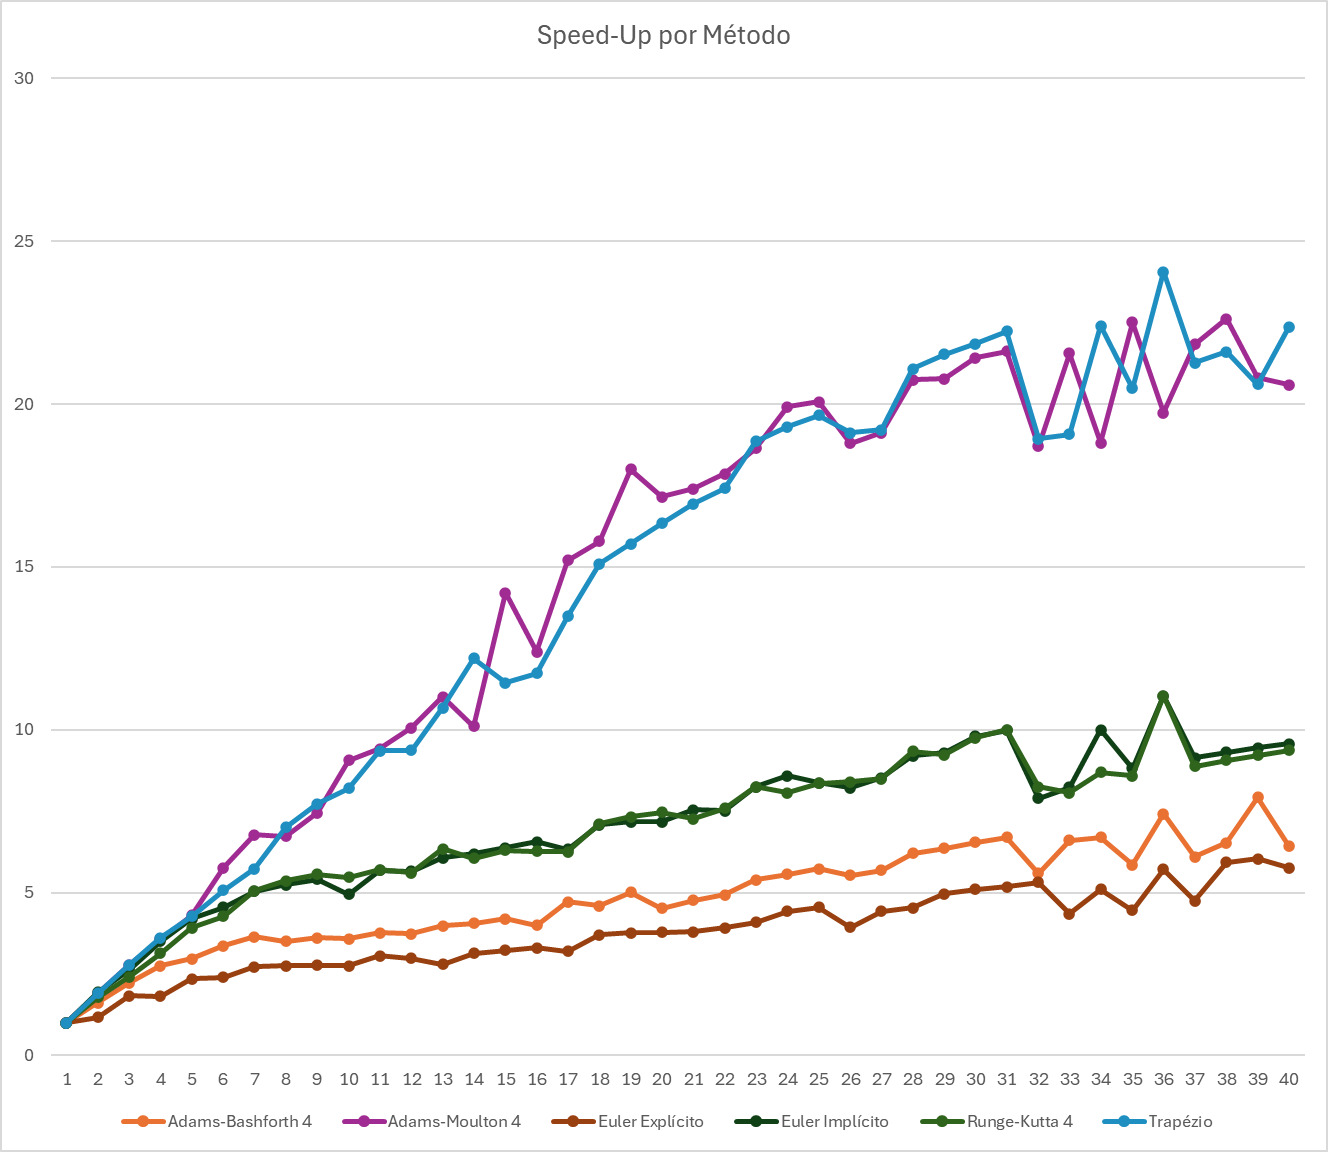
\includegraphics[width=0.7
    \linewidth]{Figuras/speedupc.jpeg}
    \caption{\textit{Speedup} por método}
    \label{fig:speedupc}
\end{figure}



\newpage
\bibliographystyle{plain}
\bibliography{references.bib}  % Add a .bib file if you have references
%\nocite{FABRICIO_ROBERTO_2025_MEC_FLU}





\end{document}


%\begin{figure} [H]
%    \centering
%    \includegraphics[width=0.65\linewidth]{name.png}
%    \caption{caption}
%    \label{fig:}
%\end{figure}